\documentclass{article}
\usepackage[utf8]{inputenc}
\usepackage[a4paper, total={6.5in, 10.5in}]{geometry}
\usepackage{merriweather}
\usepackage[hidelinks]{hyperref}
\usepackage{graphicx}
\usepackage{xcolor}
\renewcommand{\baselinestretch}{1.22} 

% for markdown inline code effect
\definecolor{bgcolor}{HTML}{E0E0E0}
\let\oldtexttt\texttt
\renewcommand{\texttt}[1]{
  \colorbox{bgcolor}{\oldtexttt{#1}}
  }
 
% % removing word break stuff
\tolerance=1
\emergencystretch=\maxdimen
\hyphenpenalty=10000
\hbadness=10000

\title{CS315: Lab Assignment 1}
\author{
  B Siddharth Prabhu\\
  \href{mailto:200010003@iitdh.ac.in}{\texttt{200010003@iitdh.ac.in}}
  }
\date{03 January 2023}

\begin{document}

\maketitle

\section{Answers for Task 1: Background}
\subsection{ping}
We use ping to check the connectivity between two computers. On running the command (here, in WSL) \texttt{ping www.google.com}, we get the round-trip time (RTT) for messages sent from the originating host to the destination computer (in this case, the web servers of google.com). On the linux terminal, such messages keep getting sent, and RTT values are displayed, until termination via Ctrl+C. On terminating this, we get statistics on the packets sent, received, and lost.

\begin{figure}[!hbt]
    \centering
    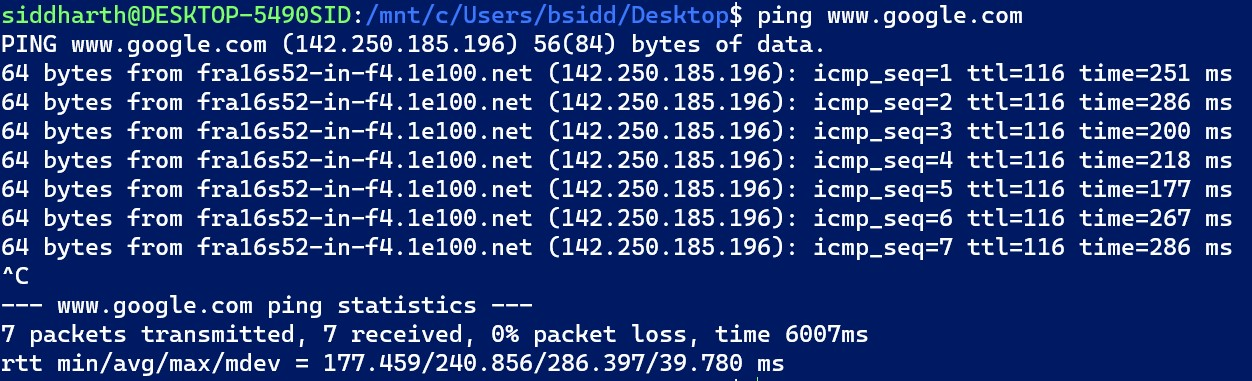
\includegraphics[scale=0.6]{q1a.jpg}
    \caption{Output for ping}
    \label{fig:my_label1}
\end{figure}

\subsection{traceroute}
We use traceroute to get the path taken to reach a host. On running \texttt{traceroute www.google.com}, we would get a report with five columns of information. The first column contains the hop number. The second column contains the IP address of the device at the given hop along the route. Then, the next three columns contain the RTT values for three signal packets that have been sent to that point (to display consistency). Note that here, the command has been adjusted according to our needs.

\begin{figure}[!hbt]
    \centering
    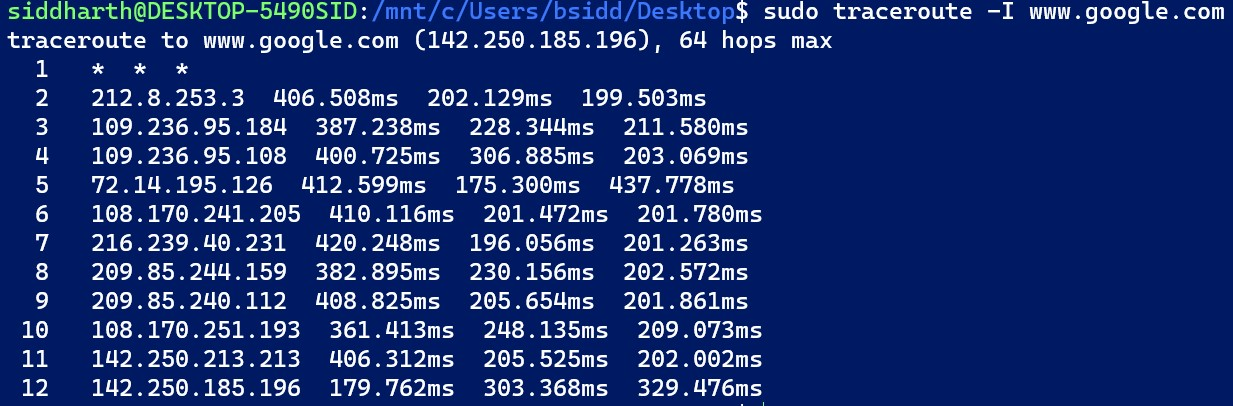
\includegraphics[scale=0.6]{q1b.jpg}
    \caption{Output for traceroute}
    \label{fig:my_label2}
\end{figure}

\newpage
\subsection{arp}
The \texttt{arp} command is used to view and modify the contents of the local ARP (Address Resolution Protocol Cache). On running the command with the \texttt{-a} flag on Windows, we can view the contents of the ARP Table, which contains details of the recently resolved MAC addresses of IP hosts on the network.

\begin{figure}[!hbt]
    \centering
    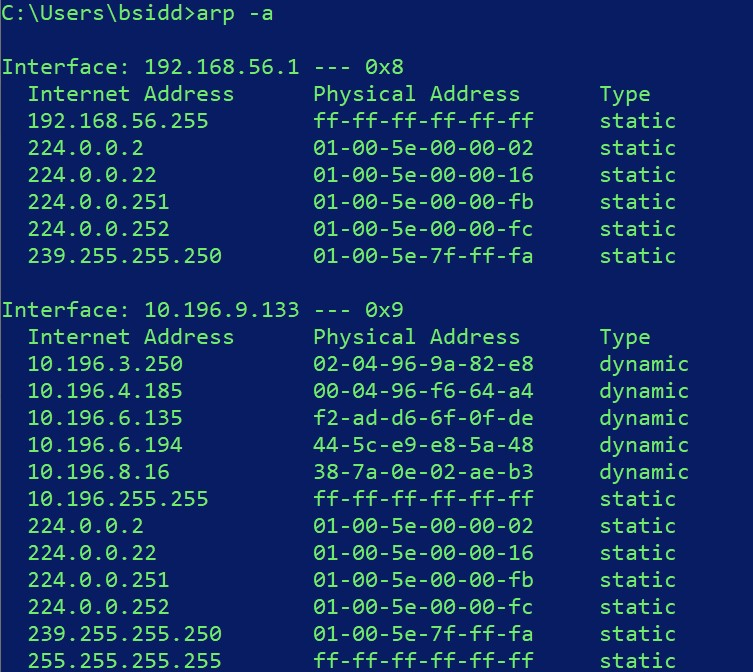
\includegraphics[scale=0.5]{q1c.jpg}
    \caption{A section of the output for arp}
    \label{fig:my_label3}
\end{figure}

\vspace{-0.75cm}
\subsection{ifconfig}
The \texttt{ifconfig} (interface configurator) utility is used for network interface configuration. Using this command, we can view the IP and MAC addresses of the different network interfaces in a system. The output from ifconfig has three main parts:
\begin{description}
    \item[Status Line] This line contains the interface name and status flags currently associated with the interface. Also, it includes MTU (Maximum Transmission Unit) and the index number of the interface. This line determines the current state of the interface. 
    \item[IP address information line] This line includes the IPv4/IPv6 address that is configured for the interface. For an IPv4 address, the configured netmask and broadcast address are also displayed.
    \item[MAC Address Line] For an IPv4 address, the third line shows the MAC address (Ethernet layer address) that is assigned to the interface. 
\end{description}
These lines are then followed by different interface statistics. 

\begin{figure}[!hbt]
    \centering
    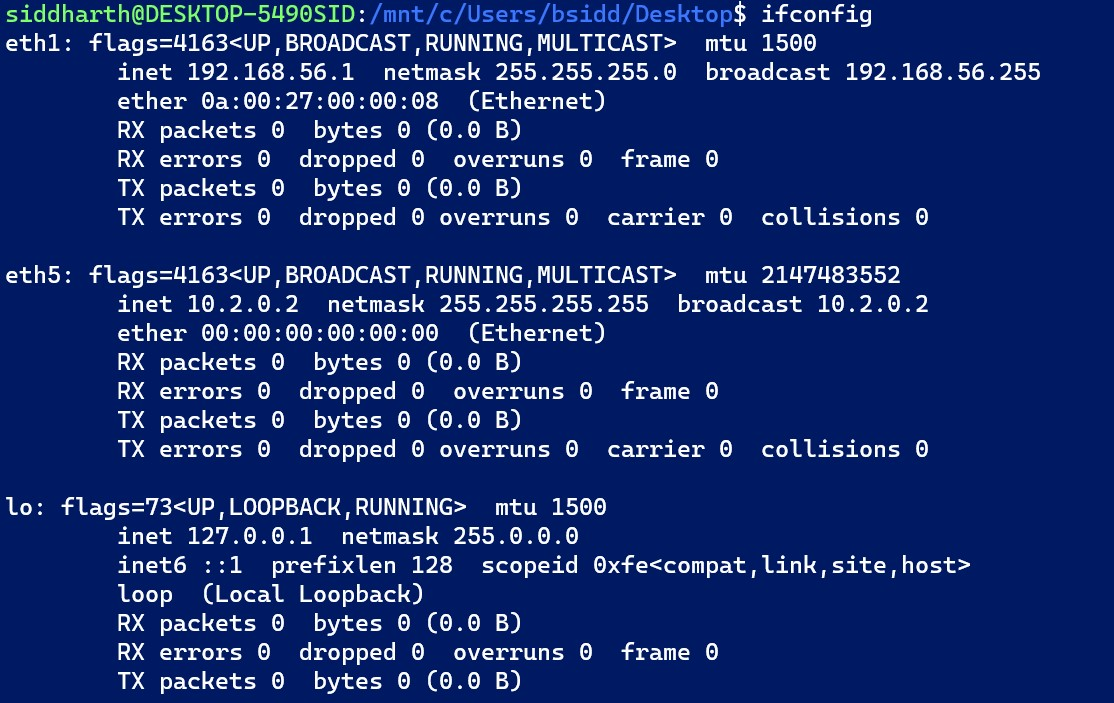
\includegraphics[scale=0.5]{q1d.jpg}
    \caption{Output for ifconfig}
    \label{fig:my_label4}
\end{figure}
\newpage

\subsection{hostname}
The \texttt{hostname} command is used to retrieve the host name of a computer or network node in a network. Hostnames are specific names or character strings that refer to a host. It is usable for the network and people.
\begin{figure}[!hbt]
    \centering
    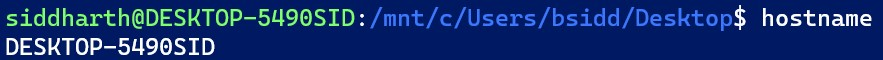
\includegraphics[scale=0.8]{q1e.jpg}
    \caption{Output for hostname}
    \label{fig:my_label5}
\end{figure}

\subsection{Review of Configuration files}
\subsubsection{\texttt{/etc/hostname}}
This file stores the system's host name, which is the FQDN (Fully Qualified Domain Name) of the system.

\subsubsection{\texttt{/etc/hosts}}
When a machine is started, it needs to know the mapping of some hostnames to IP addresses before DNS can be referenced. This mapping is kept in this particular file. In the absence of a name server, any network program on the system consults this file to determine the IP address that corresponds to a host name.

\subsubsection{\texttt{/etc/resolv.conf}}
This file a text file which is used by the resolver library that determines the IP address for a host name. This file contains the list of name servers used by the host for DNS resolution. When using DHCP (Dynamic Host Configuration Protocol), this file is populated automatically with the records issued by the DHCP Server.

\begin{figure}[!hbt]
    \centering
    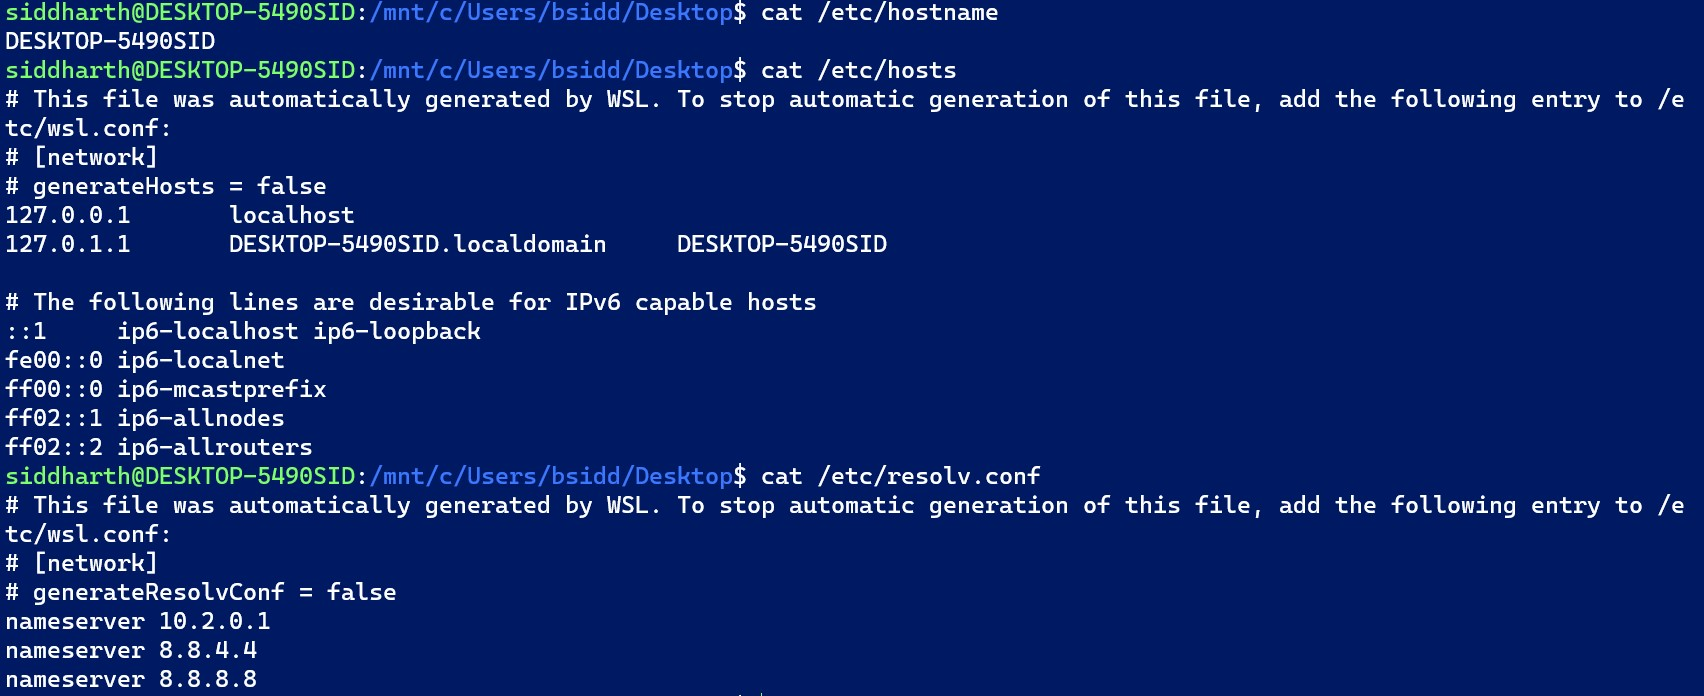
\includegraphics[scale=0.55]{q1f1.jpg}
    \caption{Contents of the hostname, hosts, and resolv.conf files}
    \label{fig:my_label1f1}
\end{figure}

\newpage
\subsubsection{\texttt{/etc/protocols}}
This file contains information regarding known protocols. For each protocol, a single line is present with information in the format: \texttt{official-protocol-name} \texttt{protocol-number} \texttt{aliases}. \# is used for comments regarding the protocols.
\begin{figure}[!hbt]
    \centering
    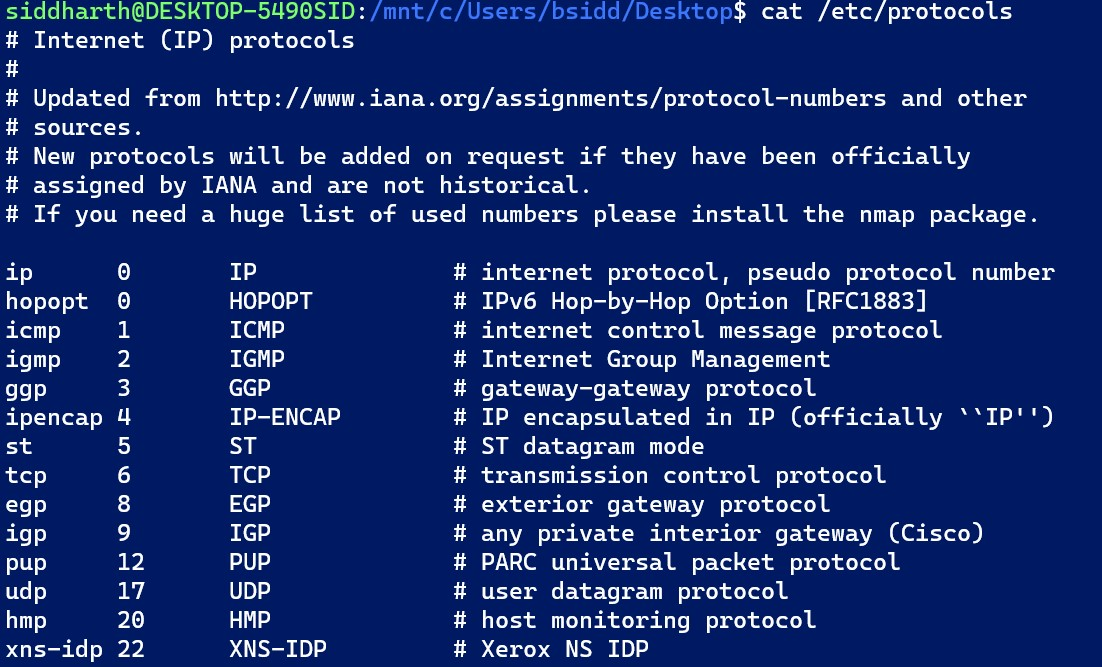
\includegraphics[scale=0.6]{q1f2.jpg}
    \caption{A section of the contents of the protocols file}
    \label{fig:my_label1f2}
\end{figure}

\subsubsection{\texttt{/etc/services}}
This file contains a list of network services, with the ports mapped to each of them. Most Internet services are assigned a specific port for their use. When a client opens a connection across the network to a server, the client uses the port to specify which service it wishes to use. This file serves as a small local database to store this information. For each service, this file specifies the service’s `well-known port number', and notes whether the service is available as a TCP (connection-oriented) or UDP (connectionless) service.

\begin{figure}[!hbt]
    \centering
    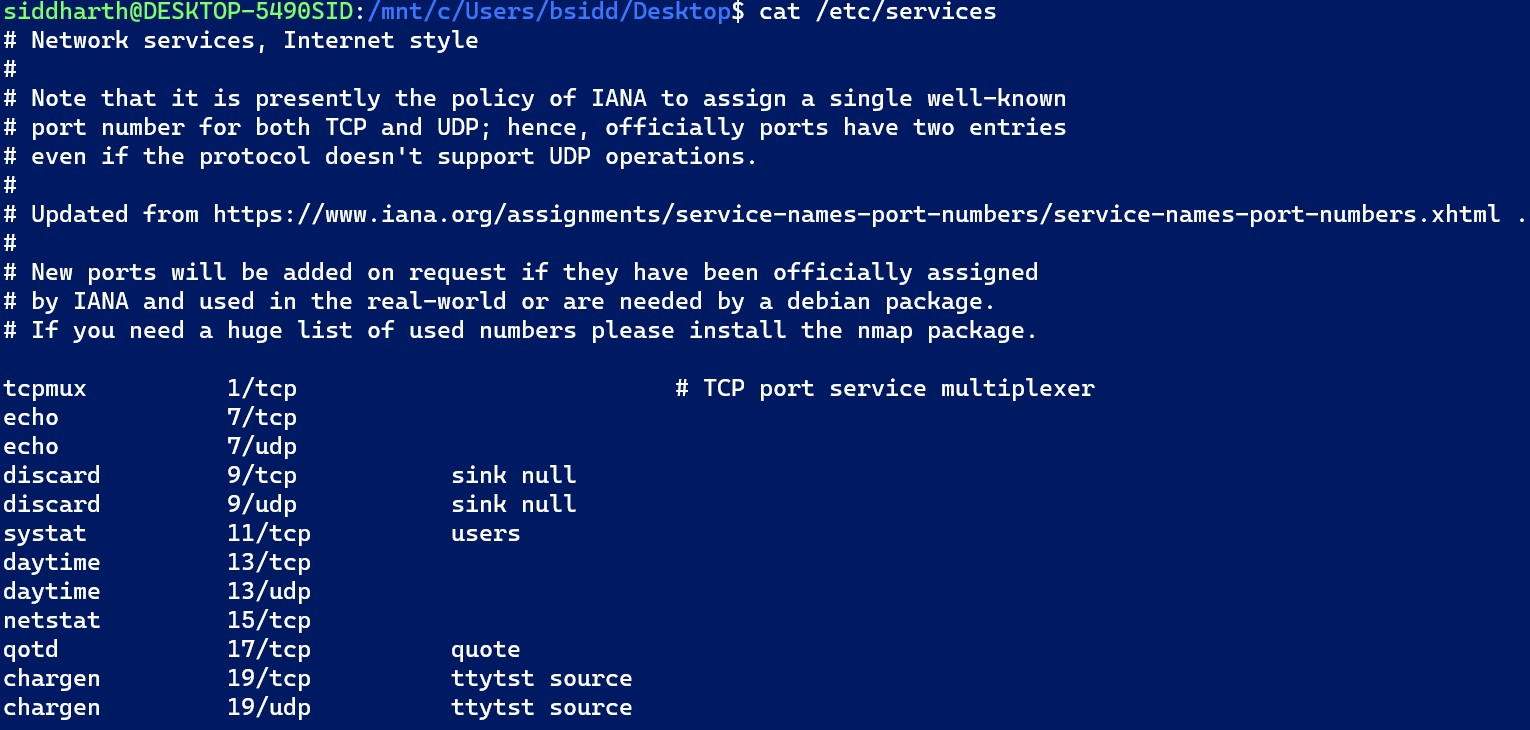
\includegraphics[scale=0.6]{q1f3.jpg}
    \caption{A section of the contents of the services file}
    \label{fig:my_label1f3}
\end{figure}

\newpage
\section{Answers for Task 2: Warm-Up Questions}
\subsection*{(i) What is your machine's hostname and IP address? How did you get this information?}
My machine's hostname is \texttt{DESKTOP-5490SID}, and the IP address assigned to it is \texttt{10.196.9.133}. The hostname was obtained via the \texttt{hostname} command, as shown in Section (1.5). The IP Address was obtained using the \texttt{ifconfig} command, next to the wifi0 label.

\begin{figure}[!hbt]
    \centering
    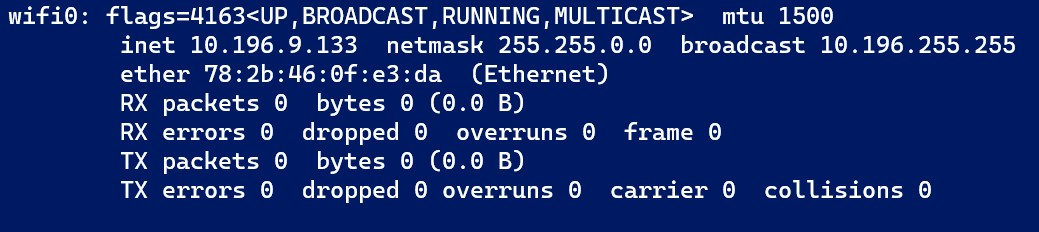
\includegraphics[scale=0.6]{q2a.jpg}
    \caption{wifi0 section of ifconfig output}
    \label{fig:my_label2a}
\end{figure}

\subsection*{(ii) What is the next hop router's IP address and MAC address? How did you get this information?}
The next hop router's IP address is \texttt{10.196.3.250}. Its MAC Address is \texttt{02:04:96:9a:82:e8}. This information is found using the \texttt{arp} command. On my Windows system, the same is done using \texttt{ipconfig} and \texttt{arp -a}.

\begin{figure}[!hbt]
    \centering
    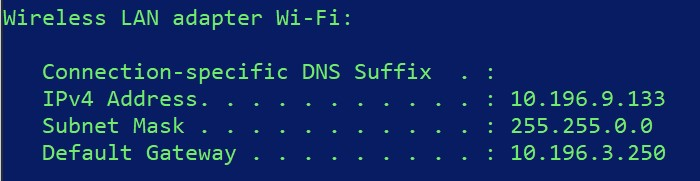
\includegraphics[scale=0.8]{q2b1.jpg}
    \caption{Default Gateway IP address obtained by ifconfig}
    \label{fig:my_label2b1}
\end{figure}
\begin{figure}[!hbt]
    \centering
    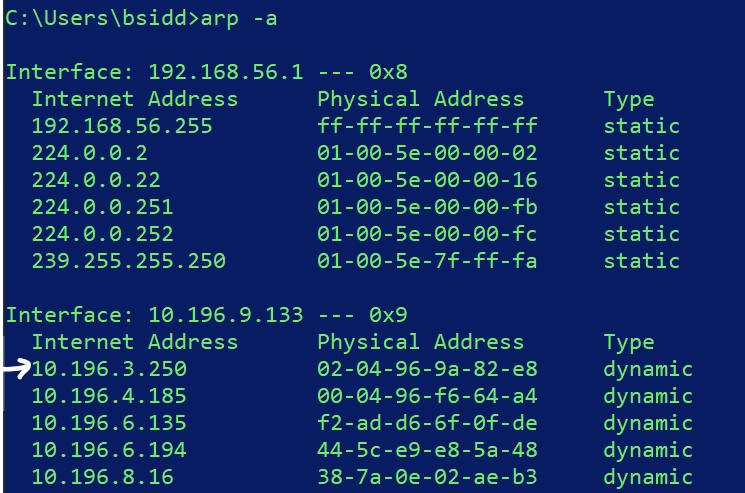
\includegraphics[scale=0.8]{q2b2.jpg}
    \caption{MAC address of the router found using arp -a}
    \label{fig:my_label2b2}
\end{figure}
\newpage

\subsection*{(iii) What is the local DNS server's IP address? How did you get this information?}
The local DNS server's IP address is \texttt{10.2.0.1}. This was obtained by looking at the contents of \texttt{/etc/resolv.conf}. 
\begin{figure}[!hbt]
    \centering
    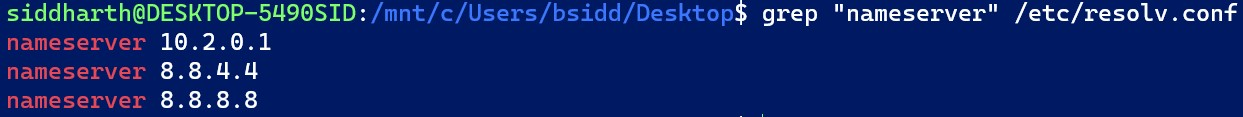
\includegraphics[scale=0.7]{q2c.jpg}
    \caption{Name Server IP Address}
    \label{fig:my_label2c}
\end{figure}

\subsection*{(iv) What do the numbers in the file /etc/protocols represent?}
The (1-byte) numbers in the file \texttt{/etc/protocols} represents the protocol number, which is used to identify the protocol.

\subsection*{(v) What is the port number associated with applications: ssh, ftp, nfs, smtp (email)? How did you get this information?}
The port numbers for the applications given are as follows:
\begin{itemize}
    \item ssh: port 22
    \item ftp: port 21
    \item nfs: port 2049
    \item smtp: 25
\end{itemize}
This is obtained using the \texttt{/etc/services} file, in combination with the grep tool.

\begin{figure}[!hbt]
    \centering
    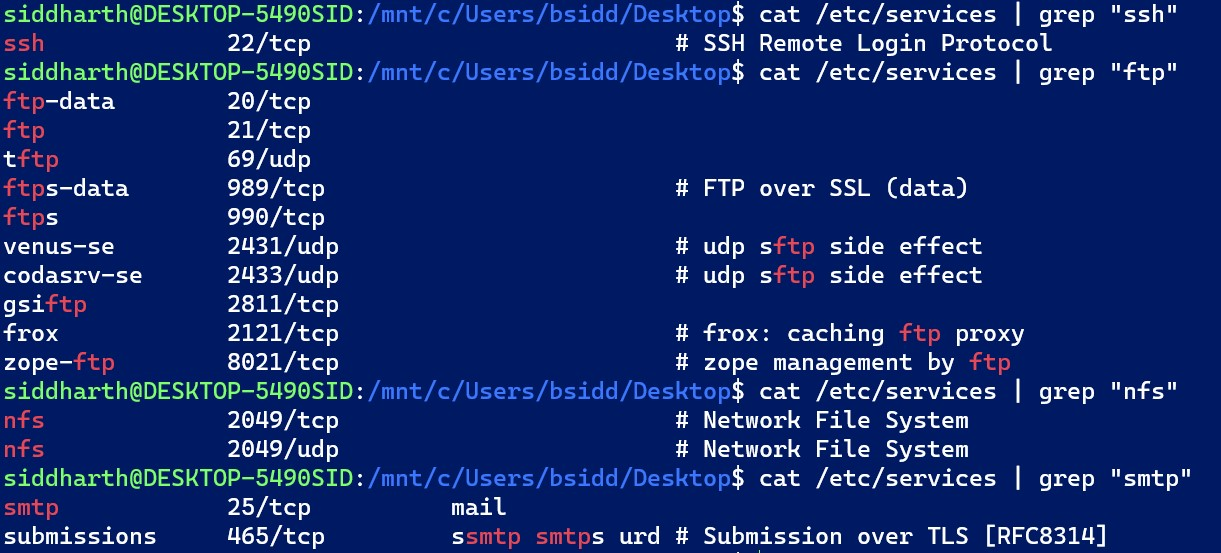
\includegraphics[scale=0.7]{q2d.jpg}
    \caption{Applications Port Numbers}
    \label{fig:my_label2d}
\end{figure}

\subsection*{(vi) How many of these questions can you answer for the phone running on android/iOS?}
In theory, we should be able to obtain all of the required answers for a phone as well. The only thing is that we would need some kind of terminal-like setup to find these things. We'd have to use some application that gets such details!

\section{Answers for Task 3}
\subsection*{(i) Using ping}
\subsubsection*{(a) Explain the results that you obtain; For example, the success and failure of the Ping}
We have obtained results of values for www.amazon.com, while not for www.iitb.ac.in, since the website may have blocked ping requests. This shows that we are able to form a connection to www.amazon.com, but not with www.iitb.ac.in.

\subsubsection*{(b) What are the reasons for the values of RTTs that you see?}
The initial value is quite high since it tries to find the path to locate the destination. The later RTT values fluctuate due to traffic and other factors. Multiple Ping requests are sent, to check consistency along the connection.

\begin{figure}[!hbt]
    \centering
    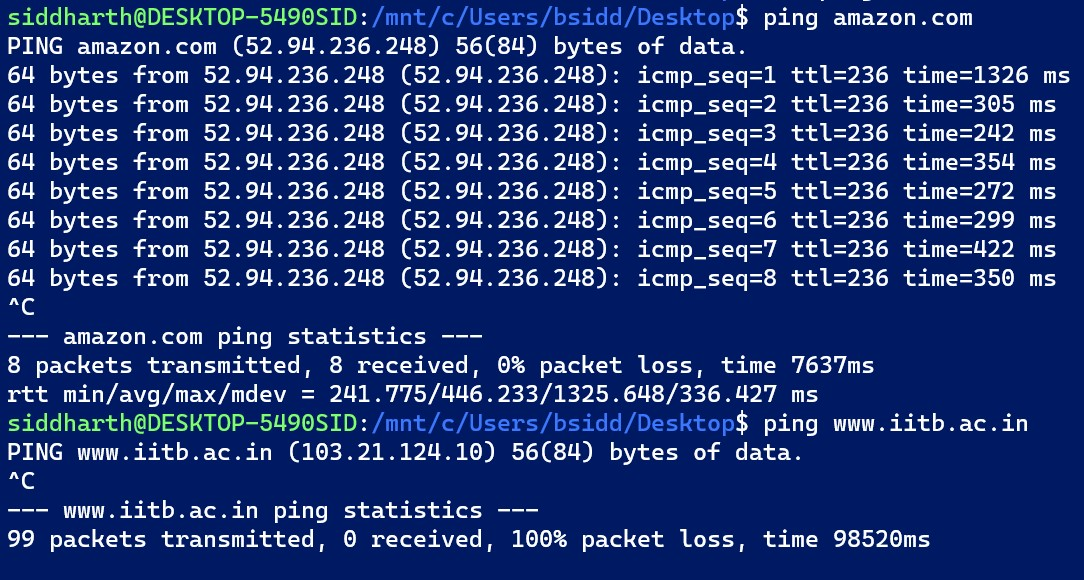
\includegraphics[scale=0.6]{q3a.jpg}
    \caption{Output of ping}
    \label{fig:my_lmnknabel2d}
\end{figure}

\vspace{-0.75cm}
\subsection*{(ii) Using traceroute}
\begin{figure}[!hbt]
    \centering
    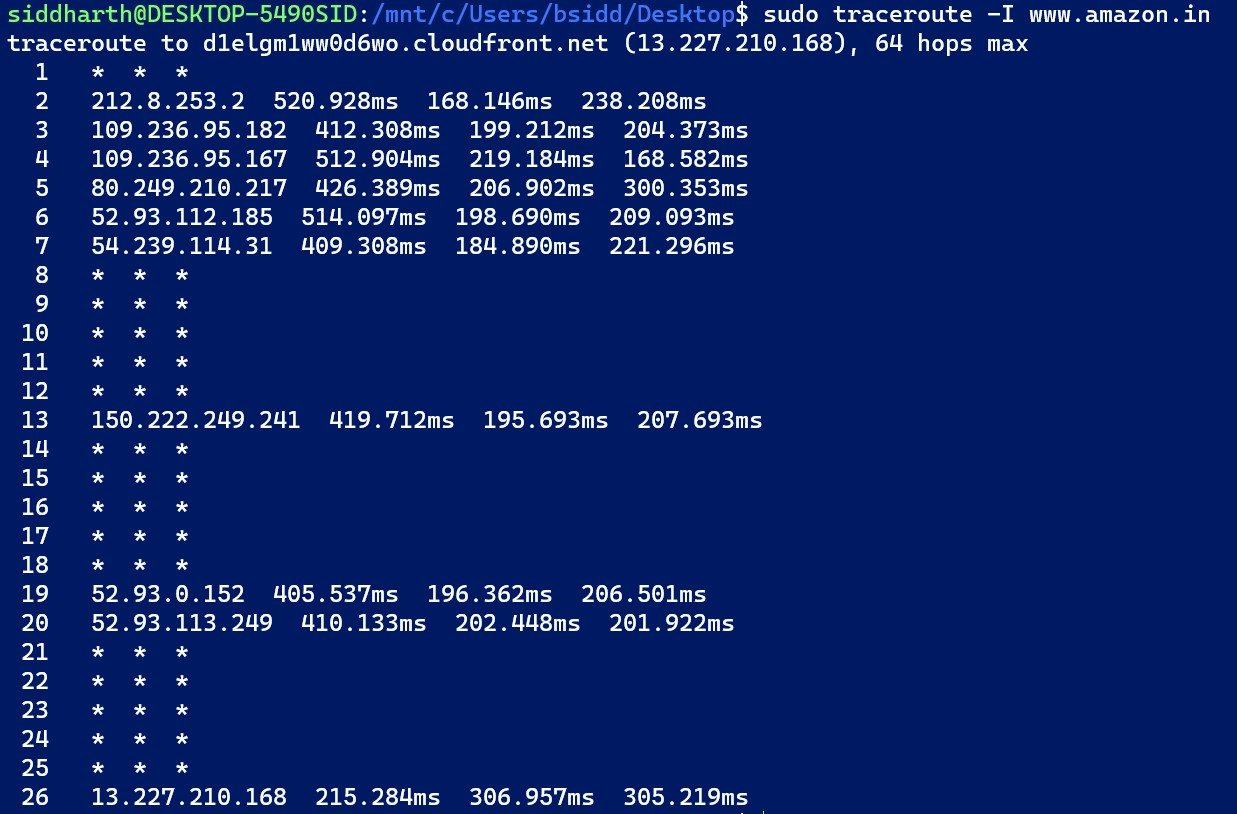
\includegraphics[scale=0.6]{q3b.jpg}
    \caption{Output of traceroute}
    \label{fig:my_labelgjj}
\end{figure}

\subsubsection*{(a) Explain what you see. Whenever successful, draw a network map from your machine to the destination, which includes the hop addresses obtained from Traceroute.}
We observe that it took 26 hops for the packet to reach www.amazon.in. A network map would look like:
10.196.9.133 (Device) $\rightarrow$ 10.196.3.250 (Next-Hop Router) $\rightarrow$
212.8.253.2  $\rightarrow$
109.236.95.182  $\rightarrow$
109.236.95.167  $\rightarrow$
80.249.210.217  $\rightarrow$
52.93.112.185  $\rightarrow$
54.239.114.31  $\rightarrow$
150.222.249.241  $\rightarrow$
52.93.0.152  $\rightarrow$
52.93.113.249  $\rightarrow$
13.227.210.168 (Destination IP)

\subsubsection*{(b) How can you change the maximum hop number?}
To do this, we can use the traceroute command along with flags \texttt{-m}, \texttt{--max-hop=num}, where num is the max hop number that we set (default is 64).

\subsubsection*{(c) What do the three timestamps signify in the result of Traceroute?}
The three timestamps signify the RTT (Round-Trip Time) values (in milliseconds) for 3 signal packets that reach a certain point in the list of hops (and return back). 

\subsubsection*{(d) What is the use of TTL (Time To Live) field in ICMP packets?}
TTL field is a counter that decreases in value after each hop of the packet. It is a time limit imposed on the data packet to be in-network before being discarded. It is an 8-bit binary value set in the Internet Protocol (IP) Header by the sending host. The purpose of a TTL is to prevent data packets from being circulated forever in the network.




\end{document}
